\Chapter{Kínai karakterek felismerése}

{\large \textbf{Az alapvonások}}

Az írásjegyek felépítésének következő lényeges szabálya az írásjegy vonásainak sorrendje. Az írásjegyek – bármilyen bonyolult legyen is némelyik – tulajdonképpen néhány igen egyszerű vonalból épülnek fel. Ezek az írásjegyek alapelemei, vagy alap-ecsetvonásai. Az alábbi képen az alapvonások néhány főbb típusa látható. Természetesen az alapvonásoknak több változata is lehetséges (méret, vastagság, irány) attól függően, hogy az írásjegy melyik részén helyezkedik el.\\

\begin{center}
	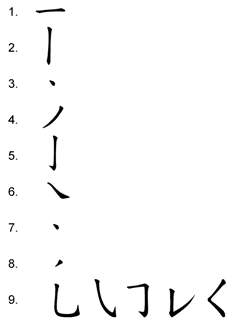
\includegraphics[scale=0.5]{chinese_strokes}
\end{center}

Minden egyes vonásnak megvan a felépítési szabálya: az ecsetvonásoknak meghatározott sorrendben kell követniük egymást, még pedig általános elvként az írásjegyek határait alkotó virtuális négyszög bal felső sarkából lefelé és jobbra haladva. Az írásjegy gerincét, fő szerkezeti elemét adó nagyobb vonást, ha az egész írásjegyet átjárja, legutoljára húzzák.\\

\newpage
{\large \textbf{A vonássorrend szabályai: }}
\begin{enumerate}
	\item A vízszintes vonások megelőzik a függőleges vonásokat.
	\item A balra lejtő vonások megelőzik a jobbra lejtő vonásokat. 
	\item Az írásjegyek írását felülről kell kezdeni. 
	\item Az írásjegyet balról jobbra haladva építik fel. 
	\item A felülről keretezett írásjegyeknél előbb a keretet kell meghúzni. 
	\item Az alulról keretezett írásjegyeknél a keretet legvégül kell meghúzni. 
	\item A teljes keretet mindig legvégül kell bezárni.
\end{enumerate}

Egy szimmetrikus felépítésű írásjegynél előbb a középső részt kell kialakítani, s csak azután az oldalakat.\\

\begin{center}
	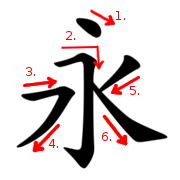
\includegraphics[scale=1.0]{vonasrend_ordered}
\end{center}

A kínai írásjegyek különböző számú alapvonásokból épülhetnek fel. Ezek közül a legegyszerűbb a csupán egyetlen vízszintes vonalból álló „egy” jelentésű \begin{CJK*}{UTF8}{gbsn}
一
\end{CJK*} ji írásjegy. A kínai írásrendszer más, egy vonásból álló írásjegyet nem tartalmaz. Aránylag ritkák a két vonásból álló írásjegyek is, például: \begin{CJK*}{UTF8}{gbsn}
二
\end{CJK*} er„kettő”,
\begin{CJK*}{UTF8}{gbsn}
十
\end{CJK*} si „tíz”,
\begin{CJK*}{UTF8}{gbsn}
人
\end{CJK*} zsen „ember” stb. A hagyományos írásjegyek zöme 15–30 vonásból épül fel (átlagosan 9 vonásból). Esetenként azonban ennél jóval több vonásból álló írásjegyek is előfordulhatnak, melyek tulajdonképpen már több önálló írásjegy összevonásának is tekinthetők. Ritkák ugyan, de léteznek 50 vagy akár 80 vonásból álló írásjegyek is.\\

{\Large OCR megvalósítások}\\

Az optikai karakterfelismerés feladata\\

A különböző formátumú dokumentumok kezelésének egyik speciális esete, amikor a kezelendő dokumentumok még nem állnak rendelkezésre elektronikus formában. Ebben az esetben szinte mindig arról van szó, hogy a dokumentumok kinyomtatva, papír alapú hordozón jelennek meg. Szövegbányászati tevékenység végzéséhez értelemszerűen digitalizálni kell a még nem digitalizált, papíron, nyomtatásban vagy írásban meglévő dokumentumokat, azaz a képként érzékelt dokumentumot szövegfájl formátumba kell átalakítani, hogy abban az után elektronikusan szerkeszthető és feldolgozható legyen. Ebben a szituációban kap szerepet az optikai karakterfelismerés (optical character recognition, OCR), amely így szövegbányászati előfeldolgozásnak tekinthető. Az optikai karakterfelismerés a mesterséges intelligencia jelfeldolgozó és generalizációs képességeit kiaknázva képes magas hatékonysággal nyomtatott, papír alapú dokumentumokon lévő karaktereket felismerni.\\

Az alap probléma itt az, hogy a nyomtatott papír alapú dokumentumok esetében nagy zajaránnyal kell megküzdeni annak érdekében, hogy a releváns információt kihámozzuk az érzékelt képi jelek és minták közül. Nyomtatott dokumentum esetében ilyen zajnak tekinthető például egy apró folt a papíron, tintaelmosódás, tintahiány, homályos háttér, apró gyűrodés a papíron, túl közeli vagy egybeolvadó betűk, betű dőlésszögének ingadozása stb. Kézírás esetén a kihívás még nagyobb, hiszen itt a személyiségjegyek sokszínűségéből adódó írásminták kavalkádjából kell kihámozni a karaktereket. Mind a nyomtatott, mind pedig a kézírásos esetben az optikai karakterfelismerő rendszer egy tanulási fázist követően képes olyanmintákat is osztályozni (a megfelelő karaktert felismerni), amelyekkel a tanulási fázisban nem találkozott, tehát megvan a szükséges generalizációs képessége.\\

Az OCR-rendszerek alapvetően két részből állnak: egyrészt a szkennelő fejből, amely a dokumentum egészét vagy részeit beszkenneli, másrészt pedig magából a mesterséges intelligencia szoftverből, ami elvégzi a beérkezett minták osztályozását, azaz magát a karakterfelismerést.\\

\begin{center}
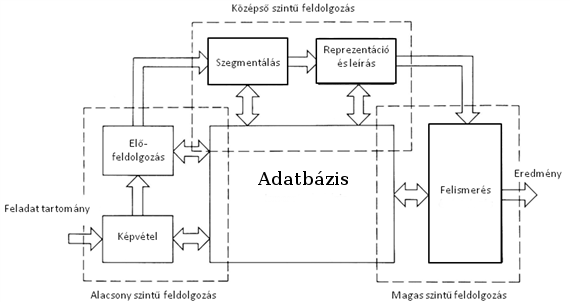
\includegraphics[scale=0.65]{ocr}
\end{center}

Szegmentáció\\

A szegmentáció során a karakterek közötti éles határ megtalálása a cél annak érdekében, hogy téves minták ne kerüljenek osztályozásra (pl. két fél karakter). A szegmentáció feladata lehet az is, hogy a karakter-dőlésszögeket, karakterméreteket normalizálja. Sok esetben a szöveges dokumentumokban nem csak karakterek vannak, hanem képek és egyéb, a felismerés szempontjából nem lényeges szimbólumok. A szegmentáció további feladata tehát az is, hogy az ilyen, számunkra nem releváns grafikus objektumok közül kiszűrje a csak karaktereket tartalmazó szöveges részeket.\\

\begin{center}
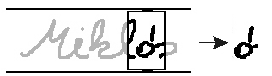
\includegraphics[scale=1.0]{ocr_segmentation}
\end{center}

Optikai előfeldolgozás\\

Az előfeldolgozás a bemeneti minta komplexitásának csökkentésére szolgál, és annak legjellemzőbb vonásait elemi ki. Különösen nagy jelentősége van a kézírás felismerésekor, ugyanis az írott betűk jóval komplexebb mintákat alkothatnak, mint a nyomtatott betűk. A jellemzőkiemelés során a komplexitás úgy csökken, hogy közben a legjellemzőbb információk megmaradnak és ezáltal a későbbi feldolgozás számításigényét redukálhatjuk. Ez a folyamat tulajdonképpen egy komplexitáscsökkentéssel járó digitalizáció. Az alábbi ábra egy egyszerű digitalizálási módszert mutat, amikor az analóg jelre egy mátrixot reprezentáló rácshálót illesztünk, és amelyik cellán átmegy az analóg karakter, az az elem a mátrixban 1 értéket vesz fel (fekete), egyéb esetben pedig 0-t (fehér).\\

\begin{center}
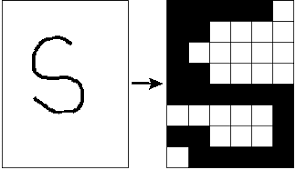
\includegraphics[scale=0.65]{ocr_preprocess}
\end{center}

Felismerés\\

Az osztályozás során történik meg a tényleges karakterfelismerés. A karakterfelismerő módszer a bemeneti jellemzővektor alapján dönti el, hogy az ismert karakterek közül melyikre hasonlít a legjobban a bemeneti vektor. Így a karakterfelismerési probléma egy asszociatív memóriát igénylő feladat, amelynek során a tárolt memóriaelemek közül kell előhívni azt, amely a bemeneti mintának legjobban megfelel.\\

Kínai karakter felismerés\\

A számítógépek képesek felismerni a karaktereket, beszélik és megértik az emberi nyelveket, kommunikálnak az emberi nyelven egyre elterjedtebb számítógépes iparban. Karakterfelismerés óriási időt takaríthat meg az adatok és üzenetek számítógépekbe történő írásához. Azonban, a kínai karakterek felismerése a számítógépen sokkal nagyobb kihívást jelent, mint a többi nyelveknél, mert hatalmas mennyiségű karakterkészlettel rendelkezik (27484 karakter).\\

A karakterek felismerése lehet online és offline karakterfelismerés. A fő különbség az, hogy az online karakterfelismerés rögzíti az ecsetvonások mozgását, míg az offline karakterfelismerés pusztán a karakter geometriai alakján alapul.\\

\begin{center}
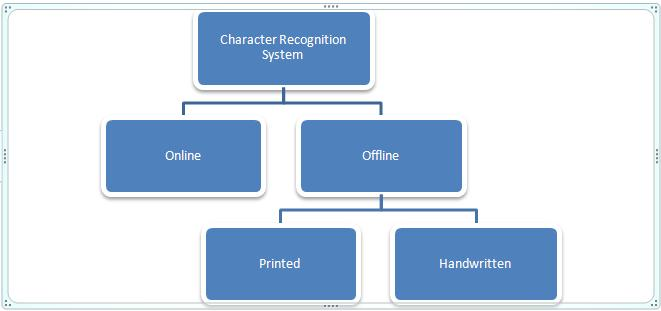
\includegraphics[scale=0.75]{ocr_online_offline}
\end{center}

Az OCR folyamatba bevitt képek általában a szkennerekből származnak, amik képet és karaktert tartalmaznak. A karakterek gyakran különböző méretűek és betűtípusokat.\\

Az előfeldolgozás során a következők jöhetnek szóba: 
\begin{itemize}
\item karakterek szétosztása a bemenetek függvényébe
\item a zaj megszüntetése
\item normalizálni a betűméretet és pozícionálni a filtert (kernel-t)
\item stroke váz generálása (thinning)
\end{itemize}

A jellemző alapú módszerek kivonják a karakter jellemzőit, mivel ezek a jellemzők matematikailag számítottak, amire alkalmas számítógép. Így az optikai karakterfelismerés (OCR) nem igazán az optikai alapokon nyugszik, hanem inkább a matematikai számításokhoz köthető.\\

Amint említettem, minden kínai karakternek egyedi geometriai alakja van, amiket a stroke-ok alakítják. A kínai karakterek felismerésének alapja a stroke-ok és a strukturális jellemzők. Hosszú ideig ez a módszer befolyásolta a kínai karakterfelismerés kutatási irányát. Azonban ez nagyon nehéz a gyakorlatban, mert a stroke és a struktúrák közötti kapcsolat nagyon instabil. A stroke-ok és a strukturális jellemzők nem tudják hatékonyan kivonni a jellemzőket vagy nem praktikus.\\

Rengeteg mód van a jellemzők kivonására, például lehet alapozni az él detektálásra, transzformációkra, rács jellemzőkre, kulcsfontosságú jellemzőkre, vektor vonali jellemzőkre.\\

\begin{center}
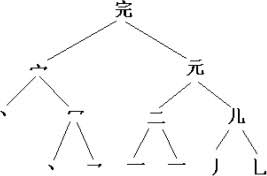
\includegraphics[scale=0.8]{ocr_features}
\end{center}

Miután rendelkezésre állnak a módszerek, amikkel ki lehet nyerni a jellemzőket, hozzáfoghatunk a végleges kimenet előállítására. Lehetséges, hogy különböző felismerési rendszereket állíthat össze és összehasonlíthatjuk a kimeneteket. Azonban ez extra számítási költséget igényel, viszont a pontosság tovább javítható.

Mikor a felismerési rendszer kimenetet generál, lehetséges, hogy néhány karakter tévesen osztályoz. Ez javítható a bemeneti képek növelésével.\\

Implementálás\\

Egy olyan algoritmust mutatok be, ami képes kínai karakterek felismerésére sok különböző betűtípussal (pl. Song, Fang, Kai, Hei, Yuan, Lishu, Weibei és Xingkai). Az algoritmus származtatott jellemzőkön alapul, és egy szótár halmazt használ. Először egy 3 szintes illesztést végez mindegyik szotárhoz képest. Az ilyen illesztésekhez kapcsolódó távolsági méréseket ezután egy központi diszkriminátorba táplálják, hogy a végső felismerési eredményt kiadják. Gyors és a pontos felismerést ért el mind a címben az összes 8 betűtípust és mind a főoldalon, amelyhez az első 4 általánosan használt betűtípus tartozik.

\begin{tabular}{ c c }
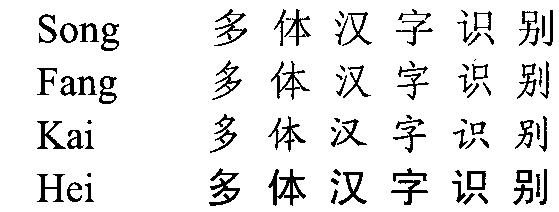
\includegraphics[scale=0.35]{chinese_fonts1} & 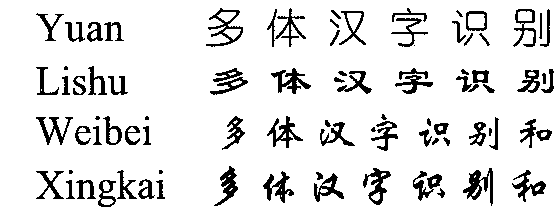
\includegraphics[scale=0.35]{chinese_fonts2}
\end{tabular}

A funkciókivonás fontos eleme az OCR-nek. Az algoritmus egy 8-dimenziós vektor tartozik [d1, d2, ... d8]. Kiszámítása: \( d_i = l_i / \sqrt{\sum_{k=1}^8 l_k^2} \)

ahol i = 1, ..., 8, és $l_i$ a csatlakoztatott fekete képpontok száma i-edik irányban.

\begin{center}
\begin{tabular}{ c c }
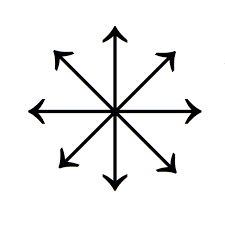
\includegraphics[scale=0.6]{8direction} & 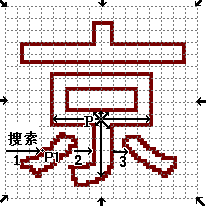
\includegraphics[scale=0.6]{ocr_PDC}
\end{tabular}
\end{center}

Az OCR rendszereknél, a felismerési algoritmusok két szakaszból állnak: tanítás és tesztelés. A hálózat súlyait a képzés során határozák meg. A képzés után a rendszer átkapcsol a tesztelési fázisra, és a szótárak szerint meghatározza a legvalószínűbb karakterindexet.

A hierarchikus illeszkedés három szintből áll. Az első szint egy osztályozó, ami felhasználja a transzformált jellemzőket. Ezután a jellemzőket egy második szintű osztályozónak adják át. Az osztályozó több elemet is kiemel (kisebb számú kimenet). A harmadik szint az összes elemet használni fogja, a karaktert a végső felismerés eredményeként kiválasztja.

A 3 szintű hierarchikus struktúra nem csak csökkenti a számítási komplexitást, hanem figyelembe veszi a jellemzők összetevőit. Az utóbbi növeli felismerési pontosság. A 3-szintű struktúra hatékonysága a felismerési arány, a sebesség és a memória használat.\\

Minden tesztet két kínai mintán végzik, összesen 7510 karakterrel. Ezek az eredmények azt mutatják, hogy a 8 betűtípus átlagos felismerési aránya 99,32\% a képzési minták esetében, pedig 98,96\%.\\

\begin{center}
\begin{tabular}{ |c|c|c|c|c|c|c|c|c|c|}
\hline
Font & Song & Fang & Kai & Hei & Yuan & Lishu & Weibei & Xingkai & Average\\
\hline
Train & 99.82 & 99.64 & 99.81 & 99.57 & 98.77 & 98.75 & 99.35 & 98.82 & 99.32\\
\hline
Test & 99.71 & 99.50 & 99.80 & 99.09 & 98.43 & 98.15 & 98.78 & 98.19 & 98.96\\
\hline
\end{tabular}
\end{center}

A kísérleti eredmények azt mutatják, hogy a javasolt algoritmus képes gyorsan és pontosan felismerni a karaktereket akár 8 különböző betűtípussal is. Az algoritmus kiváló felismerési teljesítményt nyújt a 4 leggyakrabban használt betűtípusnál.\\

!Kiegészíteni lehet CCR HANDWIRTTEN CHAR!